\documentclass{magnolia}

\magtex{tex_driver={pdftex},
        tex_packages={epigraph,xypic}}
\magfiche{document_nom={Cours Python sur la complexité},
          auteur_nom={François Fayard},
          auteur_mail={fayard.prof@gmail.com}}
\magcours{cours_matiere={python},
          cours_niveau={mpsi},
          cours_chapitre_numero={8},
          cours_chapitre={Correction}}
\magmisenpage{}
\maglieudiff{}
\magprocess

\begin{document}
%BEGIN_BOOK

\setlength\epigraphwidth{.65\textwidth}
\epigraph{\og Beware of bugs in the above code; I have only proved it correct, not tried it. \fg}{--- \textsc{Donald Knuth (1938--)}}
\hfill
\includegraphics[width=0.25\textwidth]{../../Commun/Images/python-cours-tornadoguard}
\magtoc

\section{Correction}
\subsection{Spécification d'une fonction}

La \emph{spécification} d'une fonction, c'est le contrat qu'elle doit respecter.
On peut la découper ainsi~:
\begin{itemize}
  \item \emph{Entrées :}
  \begin{itemize}
    \item \emph{Nombre et types des arguments}~: par exemple, \og cette fonction prend
          en entrée une liste $t$ d'entiers et un entier $x$ \fg.
    \item \emph{Préconditions}~: une ou plusieurs conditions qui doivent
    être vérifiées par les entrées pour que la fonction s'exécute correctement.
    Par exemple, \og les éléments de la liste doivent être distincts \fg,
          \og la liste doit être triée par ordre croissant \fg,
          \og l'entier passé en argument est positif \fg, etc.
    Si ces préconditions ne sont pas vérifiées, la fonction peut avoir un comportement
    arbitraire. Autrement dit, elle fait ce qu'elle veut, par exemple
    renvoyer un résultat arbitraire, planter, formater le disque dur,
      envoyer la totalité des images présentes sur votre ordinateur à tous vos
      contacts de messagerie, etc.
  \end{itemize}
  \item \emph{Sorties :}
  \begin{itemize}
    \item \emph{Type du résultat}~: par exemple, \og cette fonction renvoie un entier \fg,
    ou \og cette fonction renvoie un tuple formé d'un entier et d'une liste d'entiers \fg, ou
    \og cette fonction renvoie \verb!None! \fg.
    \item \emph{Valeur du résultat}~: si la fonction renvoie une \og vraie \fg valeur
          (différente de \verb!None!), que doit vérifier cette valeur~?
          Par exemple, \og la fonction renvoie $n!$ où $n$ est l'argument \fg ou
          \og la fonction renvoie une liste contenant les mêmes éléments que
          l'argument, mais triée par ordre croissant \fg.
    \item \emph{Effets secondaires} (éventuellement)~: Tous les effets que la fonction
    a sur le monde, en dehors du renvoi de son résultat. Typiquement, modification
          de l'argument ou d'une variable globale, affichage sur l'écran, suppression de toutes
          les données de l'ordinateur, envoi de missiles intercontinentaux, etc.
          Par exemple : \og après l'exécution de la fonction, le tableau passé en
          argument est trié et contient les mêmes éléments qu'au départ \fg.
  \end{itemize}
\end{itemize}
\vspace{2ex}
\begin{remarques}
  \remarque On peut regrouper \og effets secondaires \fg et \og valeur du résultat \fg 
  sous le terme
  \emph{postconditions}.
  \remarque Une fonction ne doit pas avoir d'effets secondaires autres que
  ceux apparaissant dans sa spécification. Par exemple, la fonction
  suivante n'est pas une manière acceptable de calculer le maximum
  d'un tableau.
\begin{pythoncodeline}
def apres_moi_le_deluge(t):
    """apres_moi_le_deluge(t: list[int]) -> int"""
    for i in range(1, len(t)):
        t[i] = max(t[i], t[i - 1])
    return t[-1]
\end{pythoncodeline}
En effet, son exécution ne laisse pas le système dans un état acceptable~:
\begin{pythoncode}
In [1]: [7, 2, 9, 0]

In [2]: apres_moi_le_deluge(t)
Out[2]: 9

In [3]: t
Out[3]: [7, 7, 9, 9]
\end{pythoncode}
  \remarque En pratique, on essaie souvent d'éviter les comportements totalement
  arbitraires. S'il y a un moyen simple et efficace de vérifier que
  les préconditions sont remplies, on peut préférer faire ces tests pour
  détecter un éventuel problème le plus tôt possible.
  Pour cela, on utilisera le mot clé \verb!assert! déjà utilisé pour les tests unitaires.
  Par exemple, pour une fonction calculant la factorielle, on écrit:
\begin{pythoncodeline}
def factorielle(n):
    """factorielle(n: int) -> int"""
    assert n >= 0
    f = 1
    for i in range(1, n + 1):
        f = f * i
    return f
\end{pythoncodeline}
% \begin{camlcode}
% let rec factorielle n =
%   assert (n >= 0);
%   let f = ref 1 in
%   for i = 1 to n do
%     f := !f * i
%   done;
%   !f
% \end{camlcode}
  Ainsi, un appel sur un entier $n < 0$ sera immédiatement détecté comme une
  erreur :
\begin{pythoncode}
In [1]: factorielle(-1)
(*@\textcolor{purple}{AssertionError:}@*)
\end{pythoncode}
  Sans le \verb!assert!, la fonction aurait renvoyé un résultat dénué de sens,
  1 en l'occurrence, sans se plaindre, ce qui aurait rendu l'erreur
  beaucoup plus difficile à détecter.
  \remarque Attention cependant, ce conseil n'est pas toujours possible à
  appliquer, car la précondition peut être trop couteuse, voire impossible, à
  vérifier. Par exemple, si l'on effectue une recherche dichotomique dans une liste triée, algorithme
  qui s'exécute dans le pire des cas en $\Theta(\log n)$, il serait absurde de
  vérifier que la liste est bien triée  car cette opération
  a une complexité en $\Theta(n)$. Enfin, il faut avoir conscience que ces assertions
  ne sont utiles qu'en \og production \fg et il est bien entendu inutile d'en placer dans
  un écrit de concours, sauf si cela vous est explicitement demandé.
\end{remarques}

\subsection{Correction partielle, correction totale}

\begin{definition}[nom={Terminaison d'une fonction}]
  On dit qu'une fonction \emph{termine} lorsqu'elle renvoie un résultat
  en un nombre fini d'étapes, quelles que soient les valeurs de ses
  paramètres vérifiant les préconditions.
\end{definition}


\begin{remarqueUnique}
  % \remarque Les valeurs admissibles des paramètres peuvent être limitées
  % par des préconditions : une fonction prenant en entrée un \verb!int!
  % peut n'être définie que pour les entiers positifs, une fonction
  % cherchant une occurrence d'un élément \verb!x! dans un tableau \verb!t!
  % peut se limiter au cas où \verb!x! apparait dans \verb!t!.
  \remarque Le nombre d'étapes de calcul ne sera en général pas \emph{borné},
  puisqu'il dépend de la valeur des paramètres.
\end{remarqueUnique}

\begin{exempleUnique}
\exemple
  La fonction suivante calcule $n!$ pour $n \geq 0$.
\begin{pythoncodeline}
def factorielle(n):
    """factorielle(n: int) -> int"""
    if n == 0:
        return 1
    else:
        return n * factorielle(n - 1)
\end{pythoncodeline}
  On considère qu'elle termine, car il y a une précondition $n \geq 0$.
  Cependant, si on l'appelle sur un entier $n < 0$, l'appel récursif ne termine pas.
\end{exempleUnique}

\begin{definition}[nom={Correction partielle}]
  Une fonction est dite \emph{partiellement correcte} par rapport à
  sa spécification lorsque, quelles que soient les valeurs des paramètres
  vérifiant les préconditions :
  \begin{itemize}
    \item Soit elle renvoie un résultat conforme à la spécification.
    \item Soit elle ne termine pas.
  \end{itemize}
\end{definition}

\begin{definition}[nom={Correction totale}]
  Une fonction est dite \emph{totalement correcte}, ou simplement \emph{correcte},
  si elle est partiellement correcte et qu'elle termine.
\end{definition}

\begin{exemples}

    \exemple La fonction suivante est partiellement correcte, vis-à-vis de
          n'importe quelle spécification~: il n'y a aucun risque qu'elle renvoie
          un résultat incorrect.
\begin{pythoncodeline}
def f(x):
    return f(x)
\end{pythoncodeline}
    \exemple La fonction suivante est censée calculer $x^{n}$ pour $x \in \Z$
          et $n \in \N$.
\begin{pythoncodeline}
def puissance(x, n):
    """puissance(x: int, n: int)"""
    if n == 1:
        return x
    else:
        return x * puissance(x, n - 1)
\end{pythoncodeline}
          Elle est partiellement correcte, mais pas totalement correcte :
          en effet, \verb!puissance(x, 0)! ne termine pas.

\end{exemples}

\section{Algorithme itératif}

\subsection{Terminaison}

La preuve de la terminaison d'un programme n'utilisant que des boucles \verb!for! est
immédiate. En présence de
boucles \verb!while!, prouver la terminaison peut être arbitrairement
compliqué :  ce
problème est \emph{indécidable}, c'est-à-dire qu'il n'existe pas
d'algorithme permettant de déterminer si un programme quelconque
termine. Cela n'empêche pas de montrer la terminaison
dans de nombreux cas particuliers.



\begin{definition}[nom={Variant de boucle}]
  Un \emph{variant de boucle} est une quantité :
  \begin{itemize}
    \item entière
    \item minorée
    \item qui décroit \emph{strictement} à chaque passage dans une
          boucle.
  \end{itemize}
\end{definition}

\begin{proposition}
  Si une boucle admet un variant de boucle, alors elle termine.
\end{proposition}

\begin{remarqueUnique}
  \remarque
  Une quantité entière, \emph{majorée} et qui \emph{croît} strictement
  fait aussi l'affaire.
\end{remarqueUnique}

\begin{exempleUnique}
  \exemple
  Considérons la fonction suivante.

\begin{pythoncodeline}
def log2(n):
    """log2(n: int) -> int"""
    i = 0
    x = n
    while x > 1:
        x = x // 2
        i = i + 1
    return i
\end{pythoncodeline}
% \begin{camlcode}
% let rec log2 n =
%   let i = ref 0 in
%   let x = ref n in
%   while !x > 1 do
%     x := !x / 2;
%     incr i (* équivaut à i := !i + 1 *)
%   done;
%   !i
% \end{camlcode}
  Alors $x$ est un variant de boucle.
  \begin{itemize}
    \item $\ $C'est un entier.
    \item $\ $Il est minoré par 1, tant qu'on est dans la boucle.
    \item $\ $En notant $x'$ la valeur en fin d'itération, on
          a $x' \defeq \lfloor x/2 \rfloor \leq x/2 < x$ puisque
          $x \geq 1$, donc il est strictement décroissant.
  \end{itemize}
  Cette fonction termine donc.
    Attention, si l'on remplace la condition de la boucle par
    \verb|x >= 0|, la terminaison n'est plus assurée, car la
    décroissance n'est plus stricte.
\end{exempleUnique}
\vspace{2ex}
\begin{exoUnique}
  \exo
  On considère la fonction suivante.
\begin{pythoncodeline}
def disjoints(u, v):
    """disjoints(u: list[int], v: list[int]) -> bool"""
    iu = 0
    iv = 0
    nu = len(u)
    nv = len(v)
    while iu < nu and iv < nv and u[iu] != v[iv]:
        if u[iu] < v[iv]:
            iu = iu + 1
        else:
            iv = iv + 1
    return iu == nu or iv == nv
\end{pythoncodeline}
  \begin{questions}
    \question \verb!iu! est-il un variant de boucle~? Même question pour
          \verb!iv!.
    \question Identifier un variant de boucle.
    \question Quelle précondition doit être vérifiée par \verb!u! et
    \verb!v! pour que cette fonction soit \og correcte \fg. Il faut bien sûr
    commencer par préciser ce que \emph{correcte} signifie ici, en
    s'aidant du nom de la fonction.
  \end{questions}
\end{exoUnique}
% \begin{exo}[sol]{}{}
%   On considère la fonction suivante :
% \begin{camlcode}
% let disjoints u v =
%   let iu = ref 0 in
%   let iv = ref 0 in
%   let nu = Array.length u in
%   let nv = Array.length v in
%   while !iu < nu && !iv < nv && u.(!iu) <> v.(!iv) do
%     if u.(!iu) < v.(!iv) then incr iu else incr iv
%   done;
%   !iu = nu || !iv = nv
% \end{camlcode}
%   \begin{enumerate}
%     \item \verb!iu! est-il un variant de boucle ? Même question pour
%           \verb!iv!.
%     \item Identifier un variant de boucle.
%     \item Quelle pré-condition doit être vérifiée par \verb!u! et
%     \verb!v! pour que cette fonction soit \og correcte \fg (il faut bien sûr
%     commencer par préciser ce que \emph{correcte} signifie ici, en
%     s'aidant du nom de la fonction).
%   \end{enumerate}
%   \tcblower
%   \begin{enumerate}
%     \item Lors d'un passage dans la boucle, \verb!iu! peut rester inchangé
%           (si \ml|u.(!iu) >= v.(!iv)|), donc \verb!iu! n'est ni strictement
%           croissant ni strictement décroissant : ce n'est pas un variant
%           de boucle. De même pour \verb!iv!.
%     \item À chaque passage dans la boucle, soit \verb!iu! soit \verb!iv!
%           est incrémenté et l'autre est inchangé, donc \verb!iu + iv!
%           augmente de 1 : cette quantité est strictement croissante.
%           De plus, \verb!iu + iv! est majoré par \verb!nu + nv!, donc
%           \verb!iu + iv! est un variant de boucle.
%     \item Il faut que \verb!u! et \verb!v! soient triés par ordre croissant.
%           Si c'est le cas, alors \verb!disjoints u v! renvoie \verb!true!
%           si et seulement si \verb!u! et \verb!v! n'ont aucun élément en commun.
%   \end{enumerate}
% \end{exo}

\vspace{2ex}
Les variants de boucle ne sont pas le seul outil :
fondamentalement, tout type de raisonnement peut être utilisé pour
prouver la terminaison d'une fonction.
\vspace{2ex}
\begin{exemples}
  \exemple
    Considérons la fonction ci-dessous.
\begin{pythoncodeline}
def inv_fact(n):
    """inv_fact(n: int) -> int"""
    i = 0
    f = 1
    while f < n:
        i = i + 1
        f = f * i
    return i
\end{pythoncodeline}
    Une récurrence simple montre qu'après $k$ passages
  dans la boucle, $i$ vaut $k$  et $f$ vaut $k!$.
  Comme $k! \to +\infty$,
  il est alors \og clair \fg que ce programme termine pour toute valeur de $n$.
  % On peut éventuellement remarquer que, en plus d'être clair, c'est \emph{faux} :
  %   si $n$ vaut \verb!max_int!,  il est clair (et vrai, cette fois) que le
  %   programme ne terminera pas.
  %   Cependant, on supposera sauf mention explicite du contraire
  %   que l'on travaille avec un
  %   modèle idéal des entiers dans lequel on n'a jamais de problème de
  %   dépassement de capacité.
\exemple
  Considérons maintenant le programme suivant.
\begin{pythoncodeline}
def syracuse(n):
    """syracuse(n: int) -> int"""
    k = n
    i = 0
    while k != 1:
        i = i + 1
        if k % 2 == 0:
            k = k // 2
        else:
            k = 3 * k + 1
    return i
\end{pythoncodeline}
  Si vous arrivez à montrer qu'il termine pour toute valeur de $n$,
  faites-moi signe.
  \end{exemples}

\subsection{Correction}

Les preuves de correction simples de programmes itératifs reposent sur
le principe d'\emph{invariant de boucle}, idée très similaire à celle
d'une récurrence mathématique.

\begin{definition}[nom={Invariant de boucle}]
  Un \emph{invariant de boucle} est un \emph{prédicat} $\mathcal{I}$ ayant les propriétés suivantes~:
  \begin{itemize}
    \item il est vrai avant de rentrer dans la boucle
    \item si il est vrai au début d'une itération, il reste vrai à la fin de cette itération.
  \end{itemize}
\end{definition}

\begin{remarques}
\remarque Un invariant de boucle n'a cependant aucune raison d'être vrai en milieu
  d'itération.
  \remarque Pour une boucle \emph{conditionnelle} (boucle \verb!while!) avec une
  condition $\mathcal{C}$ et un invariant $\mathcal{I}$, on commence par prouver
  que $\mathcal{I}$ est vérifié avant de rentrer dans la boucle, puis on montre
  l'hérédité, c'est-à-dire que
  $(\mathcal{C} \et \mathcal{I}) \longrightarrow \mathcal{I}$~: si la condition de boucle et l'invariant sont
  vérifiés en début d'itération, alors l'invariant est vérifié en fin
  d'itération. En sortie de boucle, $(\non \mathcal{C})$ et $\mathcal{I}$
  seront alors vrais.
\remarque Pour une boucle \emph{inconditionnelle} (boucle \verb!for!), on rédigera
  la preuve d'invariant en incorporant l'indice de boucle au prédicat.
  Pour effectuer la correction d'une boucle du type \og \verb!for k in range(a, b)! \fg, on définit les
  prédicats $\mathcal{I}_a,\ldots,\mathcal{I}_b$ et on prouve que~:
  \begin{itemize}
  \item $\mathcal{I}_a$ est vérifié avant de rentrer dans la boucle.
  \item Pour tout $k\in\interefo{a}{b}$, si $\mathcal{I}_k$ est vérifié au début de l'itération d'indice $k$, $\mathcal{I}_{k+1}$
  est vérifié en fin d'itération.
  \end{itemize}
   En sortie de boucle, $\mathcal{I}_b$ sera alors vrai.
  \remarque
  Comme pour la terminaison, les preuves de correction peuvent
  être arbitrairement difficiles~: la correction d'un programme
  peut dépendre d'une conjecture mathématique, par exemple.
  \remarque Dans les preuves, on notera souvent $x$ la valeur de la variable \verb!x! en début
    d'itération et $x'$ sa valeur en fin d'itération.
\end{remarques}

\vspace{2ex}
\begin{exempleUnique}
\exemple
  On souhaite montrer que le programme suivant renvoie bien un indice du
  minimum de $t$. Pour cela, on considère l'invariant de boucle $\mathcal{H}_i$ :
  \og $m = \min (t_0,\dots,t_{i - 1})$ et
  \verb:t[ind] = m: \fg. On note $n$ la longueur de $t$.
\begin{pythoncodeline}
def ind_min(t):
    """ind_min(t: list[int]) -> int"""
    ind = 0
    m = t[0]
    for i in range(1, len(t)):
        if t[i] < m:
            m = t[i]
            ind = i
    return ind
\end{pythoncodeline}
  \begin{itemize}
    \item $\ $$\mathcal{H}_1$ est vérifié avant de rentrer dans la boucle car
          $ind = 0$ et $m = t_0 = \min (t_0)$.
    \item $\ $Pour $1 \leq i \leq n-1$, en supposant $\mathcal{H}_i$ vraie en début
       d'itération, on a deux cas :
          \begin{itemize}
            \item
            $\ $Si $t_{i} < \min (t_0,\dots,t_{i-1}) = m$, alors
                  en fin d'itération $m'= t_{i}$ et $ind' = i$,
                  ce qui est correct puisqu'alors
                  $\min (t_{0}, \dots, t_{i}) = t_{i}$.
            \item $\ $Sinon, on a $\min (t_{0}, \dots, t_{i})
                  = \min (t_{0}, \dots, t_{i - 1}) = m = t_{ind}$.
                  Or on ne fait rien dans ce cas et l'on a donc
                  $m' = m$ et $ind' = ind$, ce qui est bien correct.
          \end{itemize}
  \end{itemize}
  À la fin de l'exécution, $\mathcal{H}_n$ est donc vraie, c'est-à-dire
  $m = \min (t_0,\dots,t_{n-1}) = \min t$ et \verb!t[ind] = m!. La variable
  \verb!ind! contient donc bien un indice du minimum de $t$.
\end{exempleUnique}

En pratique, dans un cas aussi simple, on se contentera au mieux de donner
l'invariant de boucle sans démonstration. Dans des cas plus compliqués, en
revanche, l'invariant de boucle est indispensable.

\subsection{Exemples fondamentaux}

Les deux algorithmes présentés ici sont à connaitre absolument.

\subsubsection{Exponentiation rapide, version itérative}

On considère la fonction \verb!expo(a: int, n: int) -> int!,
  dont la spécification est :
  \begin{description}
    \item \emph{Précondition}~: $n \geq 0$
    \item \emph{Résultat}~: $\verb!expo(a, n)! = a^{n}$
  \end{description}
\begin{pythoncodeline}
def expo(a, n):
    """expo(a: int, n: int) -> int"""
    p = n
    x = 1
    b = a
    while p != 0:
        if p % 2 == 1:
            x = x * b
        b = b * b
        p = p // 2
    return x
\end{pythoncodeline}
% \begin{camlcode}
% let expo a n =
%   let p = ref n in
%   let x = ref 1 in
%   let b = ref a in
%   while !p <> 0 do
%     if !p mod 2 = 1 then x := !x * !b;
%     b := !b * !b;
%     p := !p / 2
%   done;
%   !x
% \end{camlcode}
  \begin{enumerate}
    \item Montrer que $x\cdot b^{p} = a^{n}$ est un invariant de boucle.
    \item En déduire la correction partielle de la fonction.
    \item Montrer la correction totale de la fonction.
  \end{enumerate}
  % \tcblower
  % \begin{enumerate}
  %   \item
  %         \begin{description}
  %           \item[Initialisation] Au départ, on a
  %                 $x\cdot b^{p} = 1\cdot a^{n} = a^{n}$, c'est bon.
  %           \item[Hérédité] On suppose $x\cdot b^{p} = a^{n}$ et
  %                 l'on distingue les cas :
  %                 \begin{itemize}
  %                   \item si $p$ est pair, $p = 2k$, alors
  %                         \[
  %                         \begin{cases}
  %                           x' = x \\
  %                           b' = b^{2} \\
  %                           p' = k
  %                         \end{cases}
  %                         \]
  %                         On a donc $x' \cdot {b'}^{p'} = x \cdot (b^{2})^{k}
  %                         = x \cdot b^{2k} = a^{n}$, c'est bon.
  %                   \item si $p$ est impair, $p = 2k + 1$, alors
  %                         \[
  %                         \begin{cases}
  %                           x' = xb \\
  %                           b' = b^{2} \\
  %                           p' = k
  %                         \end{cases}
  %                         \]
  %                         On a donc
  %                         $x' \cdot {b'}^{p'} = xb \cdot (b^{2})^{k}
  %                         = xb^{2k + 1} = a^{n}$, c'est bon.
  %                 \end{itemize}
  %         \end{description}
  %         Donc $x\cdot b^{p} = a^{n}$ est un invariant de boucle.
  %   \item En sortie de boucle, on a $p = 0$ (condition de boucle)
  %         et $x\cdot b^{p} = a^{n}$ (invariant). On en déduit
  %         $x\cdot b^{0} = a^{n}$, c'est-à-dire $x = a^{n}$. Or la
  %         fonction renvoie $x$, elle est donc partiellement correcte.
  %   \item $p$ est un variant de boucle. En effet :
  %         \begin{itemize}
  %           \item $p$ est un entier ;
  %           \item au départ, $p = n \geq 0$ d'après la précondition ;
  %           \item si la condition de boucle est vérifiée, alors $p > 0$
  %                 et on a donc $p' = \lfloor p/2 \rfloor < p$,
  %                 et $p' \geq 0$ ;
  %           \item $p$ est donc entier, minoré par zéro et strictement
  %                 décroissant : c'est un variant de boucle.
  %         \end{itemize}
  %         Ainsi la fonction termine, donc d'après la question
  %         précédente elle est totalement correcte.
  % \end{enumerate}
% \end{exoC}
% \begin{exoC}[sol]{Recherche dichotomique}{}
% \exo

\subsubsection{Recherche dichotomique}

  On considère l'algorithme suivant :
  \begin{description}
    \item \emph{Entrées}~: un tableau $t = (t_{0}, \dots, t_{n - 1})$ et une valeur $x$
    \item \emph{Précondition}~: $t$ est trié par ordre croissant
    \item \emph{Résultat}~: un indice $i \in\interefo{0}{n}$ tel que $t_{i} = x$ s'il
          en existe un, $n$ sinon.
  \end{description}
  \begin{algorithm}[H]
    \caption{Recherche dichotomique dans un tableau trié}
  \begin{algorithmic}
      \Function{Recherche}{$x, t$}
        \State $deb \from 0$
        \State $fin \from n$
        \While{$fin - deb > 0$}
          \State $milieu \from (deb + fin) // 2$ \Comment{Division entière}
          \If{$t_{milieu} = x$}
            \State \Return{$milieu$}
          \ElsIf{$t_{milieu} < x$}
            \State $deb \from milieu + 1$
          \Else
            \State $fin \from milieu$
          \EndIf
        \EndWhile
        \State \Return{$n$}
      \EndFunction
    \end{algorithmic}
    \end{algorithm}
    \begin{figure}[H]
      \centering
      \begin{center}
        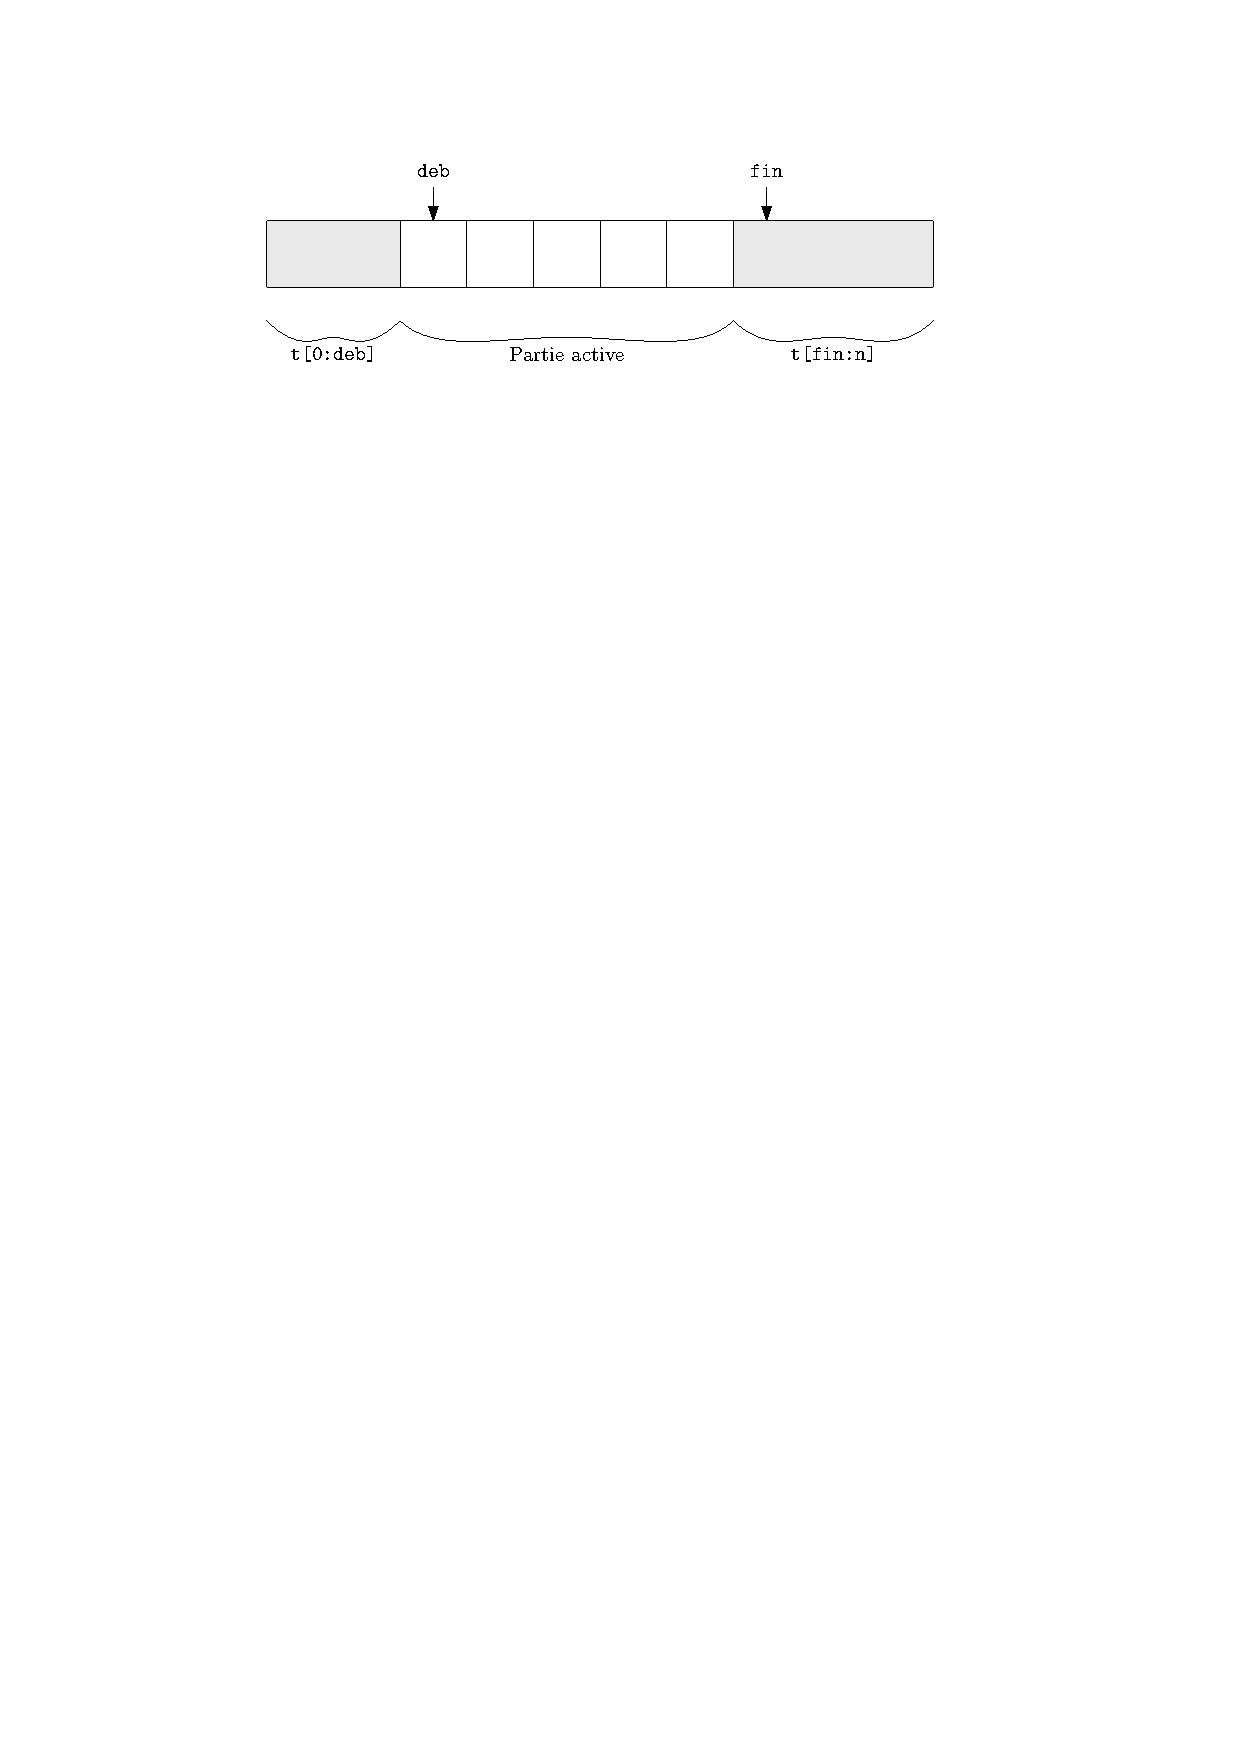
\includegraphics[scale=0.8]{../../commun/images/info-cours-correction-dichotomie.pdf}
        \end{center}
    \end{figure}
    \begin{enumerate}
      \item Montrer que cet algorithme termine.
      \item Montrer que si l'algorithme renvoie un indice $i \neq n$, alors ce
            résultat est correct.
      \item Montrer qu'on a l'invariant suivant :
            \og $x \notin t[0:deb]\ \cup\ t[fin:n]$ \fg.
      \item En déduire la correction de l'algorithme.
      \item L'algorithme reste-t-il totalement ou partiellement correct si
            \begin{enumerate}
              \item on remplace la ligne $deb \from milieu + 1$ par
                    $deb \from milieu$ ?
              \item on remplace la ligne $fin \from milieu$ par
                    $fin \from milieu - 1$ ?
            \end{enumerate}
    \end{enumerate}
  % \end{exos}
%     \tcblower
%     \begin{enumerate}
%       \item Montrons que $fin - deb$ est un variant de boucle.
%             \begin{itemize}
%               \item C'est bien un entier.
%               \item La condition de boucle assure $fin - deb > 0$ tant qu'on
%                     est dans la boucle, donc il est minoré.
%               \item On a donc $deb \leq fin - 1$, d'où
%                     $deb < \frac{deb + fin}{2} < \frac{2fin - 1}{2}$
%                     puis $deb \leq \left\lfloor\frac{deb + fin}{2} \right\rfloor \leq fin - 1$
%                     en appliquant la fonction partie entière qui est croissante
%                     (attention, les inégalités deviennent larges). Ainsi,
%                     on a $deb \leq milieu < fin$. Or :
%                     \begin{itemize}
%                       \item soit on sort de la boucle ;
%                       \item soit $deb' = milieu + 1 > deb$ et $fin' = fin$,
%                             d'où $fin' - deb' < fin - deb$ ;
%                       \item soit $deb' = deb$ et $fin' = milieu < fin$,
%                             d'où encore $fin' - deb' < fin - deb$.
%                     \end{itemize}
%                     $fin - deb$ est donc bien un variant de boucle, et la fonction
%                     termine.
%             \end{itemize}
%       \item Le seul moyen de renvoyer autre chose que $n$ est de passer le
%             test $t_{milieu} = x$ et de renvoyer $milieu$ immédiatement,
%             ce qui est évidemment correct.
%       \item
%             \begin{description}
%               \item[Initialisation] Avant la première itération, on a
%                     $deb = 0$ et $fin = n$, d'où $t[0:deb] = t[fin:n] = \emptyset$ :
%                     l'invariant est trivialement vérifié.
%               \item[Hérédité]
%                     On suppose $x \notin t[0:deb] \cup t[fin:n]$.
%                     \begin{itemize}
%                       \item Si $t[milieu] = x$, alors on sort de la fonction et
%                             la question ne se pose plus.
%                       \item Si $t[milieu] < x$, alors $x \notin t[deb:milieu + 1]$
%                             puisque le tableau est trié.
%                             Donc $x \notin t[0:deb] \cup t[deb:milieu + 1] \cup t[fin:n]
%                             = t[0:deb'] \cup t[fin:n]$.
%                       \item Si $t[milieu] > x$, alors $x \notin t[milieu:fin]$ (le
%                             tableau est trié). Donc
%                             $x \in t[0:deb] \cup t[milieu:fin] \cup t[fin:n]
%                             = t[0:deb] \cup t[fin':n]$.
%                     \end{itemize}
%             \end{description}
%             La propriété est donc bien un invariant de boucle.
%       \item Si l'on sort de la boucle sans être passé par la ligne \og renvoyer $milieu$ \fg,
%             alors on a $fin \geq deb$ et $x \notin t[0:deb] \cup t[fin:n]$, donc
%             $x \notin t$. On renvoie $n$, c'est correct. De plus, on a vu qu'un
%             résultat autre que $n$ était forcément correct et que la fonction
%             terminait : la fonction est donc correcte.
%       \item
%             \begin{enumerate}
%               \item L'algorithme reste partiellement correct après cette
%                     modification (on réduit moins l'espace de recherche,
%                     ce qui ne peut pas causer de résultat faux). En revanche,
%                     il ne termine plus, par exemple pour $x = 3$ et $t = (2)$.
%               \item Cette fois, l'algorithme termine (on réduit davantage
%                     l'espace de recherche à chaque itération). En revanche,
%                     il n'est plus correct : \textsc{Recherche(20, (10, 20, 30, 40, 50))}
%                     renvoie $5$ (il ne trouve pas l'élément) au lieu de 1.
%             \end{enumerate}
%     \end{enumerate}
% \end{exoC}



\section{Algorithme récursif}

Une première remarque s'impose : il n'y a pas de différence fondamentale
entre un programme écrit à l'aide de boucles ou de manière récursive.
En effet, il est facile de remplacer toutes les boucles \verb!while!
par des récursions, et toujours possible, mais pas facile en règle
générale,
de remplacer la récursion par une boucle \verb!while!. En un
certain sens, tout ce qui a été dit sur les programmes itératifs
s'applique donc aux programmes récursifs, en particulier le caractère
arbitrairement difficile des preuves de terminaison.

\subsection{Principe général}

En première approche, la terminaison d'un programme récursif repose sur
l'existence d'un certain nombre, potentiellement infini, de cas de base
et sur la certitude que toute suite d'appels finit par arriver sur l'un
de ces cas de base.\\

Le cas le plus simple et le plus fréquent est celui d'un programme ayant
une définition de ce type :
\begin{itemize}
  \item $f(0)$ est donné.
  \item $\forall n \in \N, \ f(n+1)\defeq g(n,f(n))$ où $g$ est une fonction
  que l'on sait calculer.
\end{itemize}
Il est alors immédiat de prouver la terminaison par récurrence, et souvent
possible de prouver simultanément la correction.
\vspace{2ex}
\begin{exoUnique}
  \exo
  Montrer que le programme suivant termine et calcule $n!$, pour tout
  entier $n \geq 0$.
\begin{pythoncodeline}
def factorielle(n):
    """factorielle(n: int) -> int"""
    if n == 0:
        return 1
    else:
        return n * factorielle(n - 1)
\end{pythoncodeline}
% \begin{camlcode}
% let rec fact n =
%   if n = 0 then 1 else n * fact (n - 1)
% \end{camlcode}
  % \tcblower
  % Posons $H(n)$ : \og \verb!fact n! termine et renvoie $n!$ \fg.
  % \begin{description}
  %   \item[Initialisation] \verb!fact 0! termine en renvoyant 1,
  %         et $0! = 1$, c'est bon.
  %   \item[Hérédité] On suppose $H(n)$ pour un certain $n \geq 0$.
  %         On a alors \verb!fact (n + 1) = n * fact n! d'après
  %         le code. Or \verb!fact n! termine et renvoie $n!$,
  %         donc \verb!fact (n + 1)! termine et renvoie
  %         $(n + 1)\cdot n! = (n + 1)!$.
  % \end{description}
  % On conclut donc que pour tout $n \geq 0$, l'appel \verb!fact n!
  % termine et renvoie $n!$.
\end{exoUnique}
% \begin{exo}[sol]{}{}
% \end{exo}

Fondamentalement, ce qui rend possible la récurrence est la décroissance
stricte de l'argument au cours des appels récursifs.
Comme $\N$ n'admet pas de suite infinie strictement décroissante,
on peut alors conclure que la suite des appels se termine. En pratique,
on justifiera cette décroissance et l'on ne rédigera pas la récurrence.
C'est l'équivalent d'un variant de boucle
dans un programme impératif.\\

La correction d'un programme récursif est parfois nettement plus simple
à prouver que celle d'un programme itératif équivalent. En effet, la
correspondance entre le code et les identités mathématiques qui le
justifient peut apparaitre beaucoup plus clairement dans le cas
récursif.

% \begin{exempleC}{Exponentiation rapide, version récursive}{}
\begin{pythoncodeline}
def expo(x, n):
    """expo(x: int, n: int) -> int"""
    if n == 0:
        return 1
    else:
        if n % 2 == 0:
            return expo(x * x, n // 2)
        else:
            return x * expo(x, n - 1)
\end{pythoncodeline}
  \begin{itemize}
    \item Si $n>0$, $0 \leq n - 1 < n$ et $0 \leq n/2 < n$, donc $n$ décroit
    strictement au cours des appels jusqu'à être nul : la fonction termine.
    \item Les identités $x^0 = 1$, $x^{2k} = (x^2)^k$ et
    $x^n = x\cdot x^{n - 1}$ si $n \geq 1$ sont correctes, donc la
    fonction aussi.
  \end{itemize}
% \end{exempleC}

\vspace{2ex}
Il arrive souvent que la suite des arguments ne soit
pas strictement décroissante, soit parce que cela n'a pas de sens, soit parce que c'est simplement faux.
Dans ce cas, on peut chercher une fonction $\phi$ de l'ensemble des
arguments dans $\N$ dont les valeurs décroissent strictement au cours des
appels successifs. Autrement dit,
on cherche une fonction $\phi$ à valeurs dans $\N$ telle que, dès que le
programme $f$ contient un appel du type $f(x) \to f(y)$, on ait
$\phi(y) < \phi(x)$.
\vspace{2ex}
% \begin{exo}[sol]{}{}
\begin{exoUnique}
\exo
  Justifier la terminaison de la fonction suivante.
\begin{pythoncodeline}
def f(n):
    """f(n: int) -> int"""
    if n % 2 != 0 or n == 0:
        return n
    else:
        return f((3 * n) // 2)
\end{pythoncodeline}
% \begin{camlcode}
% let rec f n =
%   if (n mod 2 <> 0) || (n = 0) then n
%   else f (3 * n / 2)
% \end{camlcode}
  % \tcblower
  % Il faut considérer l'exposant de 2 dans la décomposition en
  % facteurs premiers de $n$ (ce qu'on appelle la $2$-\emph{valuation}
  % de $n$), que l'on va noter $\phi(n)$.
  % \begin{itemize}
  %   \item Si $n$ est impair ou nul, la fonction termine immédiatement.
  %   \item Sinon, on a $n = 2k$ avec $\phi(k) = \phi(n) - 1$ et
  %         $\phi\left(\frac{3n}{2}\right) = \phi(3k) = \phi(k) = \phi(n) - 1$.
  %   \item Ainsi, $\phi(n)$ est un entier naturel qui décroit strictement
  %         au cours des appels et la fonction termine quand il atteint zéro :
  %         on peut conclure que la fonction termine.
  % \end{itemize}
\end{exoUnique}
% \end{exo}



%END_BOOK
\end{document}